 \documentclass[write-up.tex]{subfiles}
\begin{document}
\begin{appendices}

\section{C++ code}
\begin{lstlisting}
#include <imgui-SFML.h>
#include <SFML/Window/Mouse.hpp>
#include <imgui.h>
#include <SFML/System/Vector2.hpp>
#include <SFML/Graphics.hpp>
#include<iostream>
#include <algorithm>
#include<vector>
#include<cmath>
#include <omp.h>

using namespace std;

static int particle_num = 1600;
static float particle_mass = 30.f;
const int particle_radius = 5;
const float collision_damping = 0.8f;
const float pi = 3.141f;
static float target_density = 100.f;
static float pressure_multiplier = 75.f;
static float smoothing_radius = 70.f;
const float dt = 1.f/60.f;
static float gravity = 0.f;
static int framerate = 60;
static int viscosity_strength = 10.f;
static bool interactive = false;

struct particle{
    sf::CircleShape droplet{particle_radius};
    sf::Vector2f position{0.f, 0.f};
    sf::Vector2f velocity{0.f, 0.f};
    float local_density = 1.f;
    float local_pressure = 1.f;
    sf::Vector2f predicted_position{0.f, 0.f};
};

vector<particle> particles(particle_num);


void placeParticles(){
    int particlesPerRow = sqrt(particle_num);
    int particlesPerColumn = (particle_num - 1)/particlesPerRow + 1;
    int spacing = 2.5*particle_radius;
    for (int i = 0; i < particle_num; i++){
        particles[i].position.x = (i % particlesPerRow + particlesPerRow / 2.5f +0.5f) * spacing;
        particles[i].position.y = (i / particlesPerRow + particlesPerColumn / 2.5f +0.5f) * spacing;
    }
}

void resolveGravity(int i){
    particles[i].velocity.y += gravity * dt;
}

void predictPositions(int i){
    particles[i].predicted_position.x = particles[i].position.x + particles[i].velocity.x * dt;
    particles[i].predicted_position.y = particles[i].position.y + particles[i].velocity.y * dt;
}

float smoothingKernel(double dst){
    float volume = pi * (float)(pow(smoothing_radius, 4.0)/2);
    if (dst >=smoothing_radius){
        return 0.f;
    }
    float value = (float)pow(smoothing_radius - dst, 3);
    return value/volume;
}
float smoothingKernelDerivative(double dst){
    if (dst >= smoothing_radius) return 0.0;
    float value = -6.f * (smoothing_radius - dst) * (smoothing_radius - dst) / (pi * pow(smoothing_radius, 4));
    return value;
}
float calculateDensity(int i){
    float density = 0.f;
    for (int j =0; j < particle_num; j++){
        float dst = sqrt((particles[j].predicted_position.x - particles[i].predicted_position.x) * (particles[j].predicted_position.x - particles[i].predicted_position.x)  + (particles[j].predicted_position.y - particles[i].predicted_position.y) * (particles[j].predicted_position.y - particles[i].predicted_position.y));
        float influence = smoothingKernel(dst);

        density += particle_mass * influence;
    }
    return density;
}

float densityToPressure(int j){
    float density_error = particles[j].local_density - target_density;
    float local_pressure = density_error * pressure_multiplier;
    return local_pressure;
}

float sharedPressure(int i, int j){
    float pressurei = densityToPressure(particles[i].local_density);
    float pressurej = densityToPressure(particles[j].local_density);
    return (-(pressurei + pressurej) / 2.f);
}

sf::Vector2f calculatePressureForce(int i){
    sf::Vector2f pressure_force;
    sf::Vector2f viscosity_force;
    for (int j = 0; j<particle_num; j++){
        if (i == j) continue;
        float x_offset;
        float y_offset;
        if (particles[i].predicted_position == particles[j].predicted_position){
            x_offset = (float)1+ (rand() % 20);
            y_offset = (float)1+ (rand() % 20);
        }
        else{
            x_offset = particles[j].predicted_position.x - particles[i].predicted_position.x;
            y_offset = particles[j].predicted_position.y - particles[i].predicted_position.y;
        }
        double dst = sqrt(abs(x_offset * x_offset + y_offset * y_offset));
        float gradient = smoothingKernelDerivative(dst);
        float x_dir = x_offset/dst;
        float y_dir = y_offset/dst;
        // Newton's 3rd law implementation below
        float shared_pressure = sharedPressure(i, j);
        pressure_force.x += shared_pressure * gradient * particle_mass/particles[j].local_density * x_dir;
        pressure_force.y += shared_pressure * gradient * particle_mass/particles[j].local_density * y_dir;
    }
    return pressure_force;
}

sf::Vector2f calculateViscosityAcceleration(int i){
    sf::Vector2f viscosity_acceleration;
    float dst;
    for (int j; j<particle_num; j++){
        if (i==j) continue;
        dst = sqrt((particles[i].predicted_position.x - particles[j].predicted_position.x) * (particles[i].predicted_position.x - particles[j].predicted_position.x) + (particles[i].predicted_position.y - particles[j].predicted_position.y) * (particles[i].predicted_position.y - particles[j].predicted_position.y));
        viscosity_acceleration.x -= (particles[i].velocity.x - particles[j].velocity.x) * (smoothingKernel(dst)) * viscosity_strength;
        viscosity_acceleration.y -= (particles[i].velocity.y - particles[j].velocity.y) * (smoothingKernel(dst)) * viscosity_strength;
        if (viscosity_acceleration.x > 0 || viscosity_acceleration.y > 0){
            viscosity_acceleration.x = 0;
            viscosity_acceleration.y = 0;
        }
    }
    return viscosity_acceleration;
}

void resolveCollisions(int i, sf::Vector2u window_size){
    if (particles[i].position.x > window_size.x || particles[i].position.x < 0){
        particles[i].position.x = clamp((int)particles[i].position.x, 0, (int)window_size.x);
        particles[i].velocity.x *= -1;
    }
    if (particles[i].position.y >= window_size.y || particles[i].position.y <= 0){
        particles[i].position.y = clamp((int)particles[i].position.y, 0, (int)window_size.y);
        particles[i].velocity.y *= -1;
    }
}

void resolveColour(int i, float vel){
    int b = clamp((int)(-255/50 * vel + 255), 0, 255);
    int r = clamp((int)(255/50 * vel -255), 0, 255);
    int g = clamp((int)(-abs(255/50 * (vel-50))+255), 0, 255);
    particles[i].droplet.setFillColor(sf::Color(r, g, b));
}

sf::Vector2f interactiveForce(sf::Vector2i position, int i, float repulsive){
    sf::Vector2f force;
    float dst = (particles[i].position.x - position.x) * (particles[i].position.x - position.x) + (particles[i].position.y - position.y) * (particles[i].position.y - position.y);
    if (dst<=10000){
        force += (((sf::Vector2f)position) - particles[i].predicted_position) * (100-sqrt(dst))/4.f * repulsive;
    }
    return force;
}

int main()
{
    //Initialize SFML
    sf::RenderWindow window(sf::VideoMode(900, 900), "Smoothed Particle Hydrodynamics Simulation");
    window.setFramerateLimit(framerate);
    sf::View view = window.getDefaultView();
    sf::Vector2u window_size = window.getSize();
    placeParticles();
    ImGui::SFML::Init(window);
    sf::Vector2i position;
    float repulsive = 1;
    sf::Clock deltaClock;
    while (window.isOpen())
    {
        sf::Event event;
        while (window.pollEvent(event))
        {
            ImGui::SFML::ProcessEvent(event);
            if (event.type == sf::Event::Closed)
                window.close();
            if (event.type == sf::Event::Resized){
                sf::FloatRect visibleArea(0.f, 0.f, event.size.width, event.size.height);
                window.setView(sf::View(visibleArea));
            }
            if (event.type == sf::Event::MouseButtonPressed){
                interactive = true;
                if (event.mouseButton.button == sf::Mouse::Left){
                    repulsive = 1.f;
                }
                else{
                    repulsive = -1.f;
                }

            }
            if (event.type == sf::Event::MouseButtonReleased){
                interactive = false;
            }
        }
        sf::Vector2u window_size = window.getSize();
        ImGui::SFML::Update(window, deltaClock.restart());
        window.clear();

        //ImGui Menu
        ImGui::Begin("Menu");
        ImGui::SliderInt("Particle Num", &particle_num, 1, 1600);
        ImGui::SliderFloat("Particle Mass", &particle_mass, 10.f, 100.f);
        ImGui::SliderFloat("Target Density", &target_density, 0.f, 500.f);
        ImGui::SliderFloat("Pressure Multiplier", &pressure_multiplier, 0.f, 1000.f);
        ImGui::SliderFloat("Smoothing Radius", &smoothing_radius, 10, 200);
        ImGui::SliderFloat("Gravity", &gravity, 0.f, 100.f);
        ImGui::End();
        sf::CircleShape circle;
        position =  sf::Mouse::getPosition(window);
        for (int i = 0; i < particle_num; i++){
            resolveCollisions(i, window_size);
            //gravity step
            resolveGravity(i);
            //Predict next positions
            predictPositions(i);
            // window bounding box
            //calculate densities
            particles[i].local_density = calculateDensity(i);
            //convert density to pressure
            particles[i].local_pressure = densityToPressure(i);
            //Calculate pressure forces and acceleration
            sf::Vector2f pressure_force = calculatePressureForce(i);
            if (interactive){
                pressure_force += interactiveForce(position, i, repulsive);
            }
            sf::Vector2f pressure_acceleration;
            pressure_acceleration.x = pressure_force.x/particles[i].local_density;
            pressure_acceleration.y = pressure_force.y/particles[i].local_density;
            //Calculate acceleration due to viscosity
            pressure_acceleration += calculateViscosityAcceleration(i);
            particles[i].velocity.x += pressure_acceleration.x * dt;
            particles[i].velocity.y += pressure_acceleration.y * dt;
            //resolve colour
            float vel = sqrt(particles[i].velocity.x * particles[i].velocity.x + particles[i].velocity.y * particles[i].velocity.y);
            resolveColour(i, vel);// add at the end
            //calculate particle positions with radius offset
            particles[i].position.x += particles[i].velocity.x * dt;
            particles[i].position.y += particles[i].velocity.y * dt;
            //set particle position on screen
            particles[i].droplet.setPosition(particles[i].position.x+particle_radius, particles[i].position.y+particle_radius);
            //render particle
            window.draw(particles[i].droplet);
        }
        ImGui::SFML::Render(window);
        window.display();

    }
     ImGui::SFML::Shutdown();

    return 0;
}
\end{lstlisting}

\pagebreak

\section{Media}
\label{appendix:a}
\begin{figure}[h]
\centering
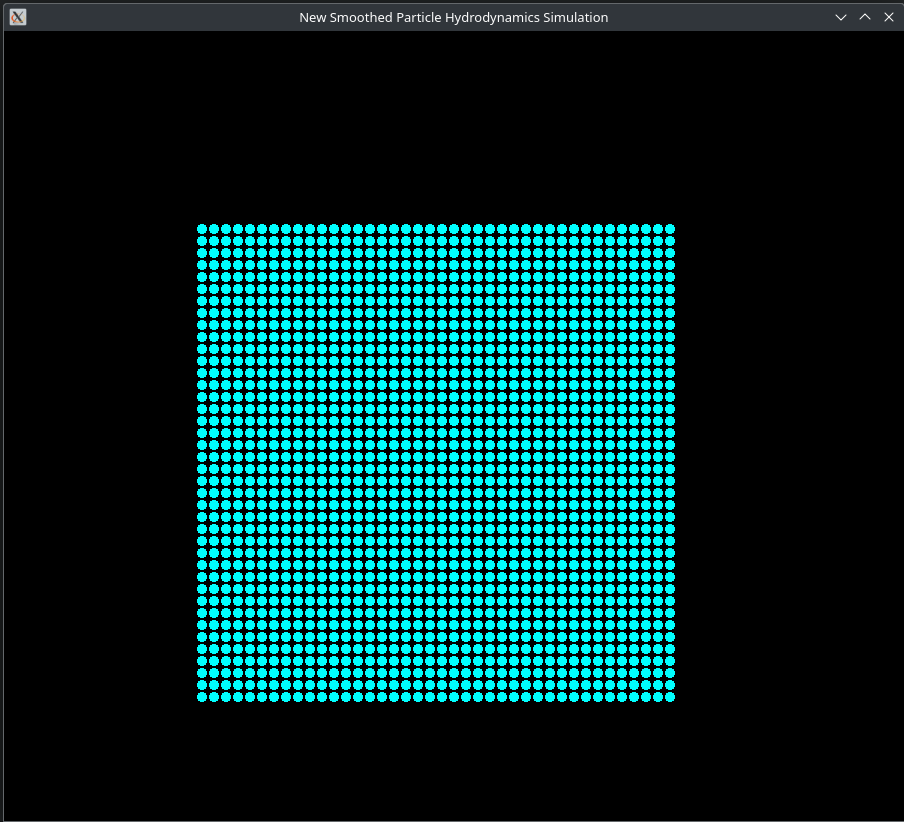
\includegraphics[width=0.6\textwidth]{more_still_particles_19-05-24.png}
\caption{Cyan particles rendered on screen.}
\label{fig:cyan}
\end{figure}

\begin{figure}[h]
\centering
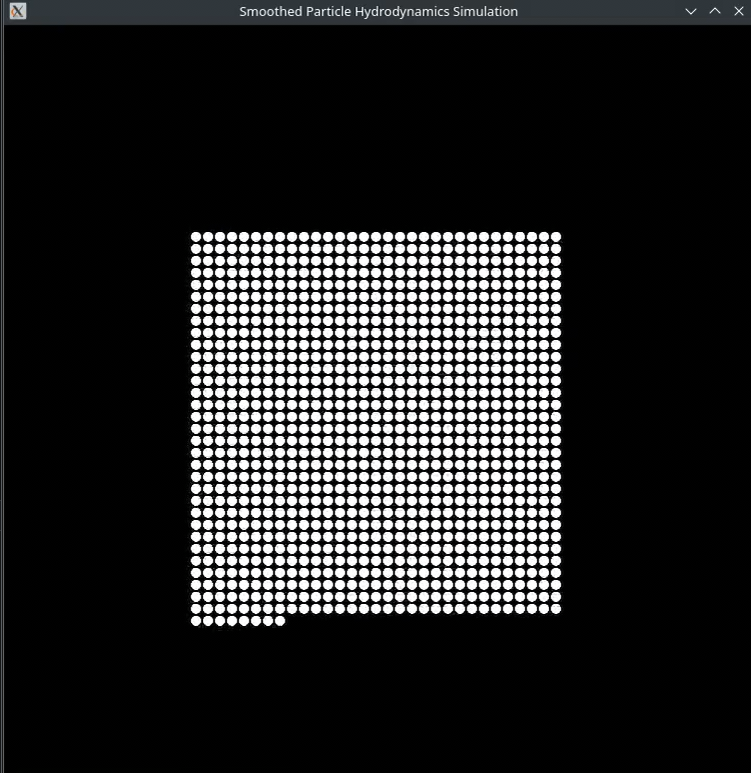
\includegraphics[width = 0.3\textwidth]{no_collision_f1.png}
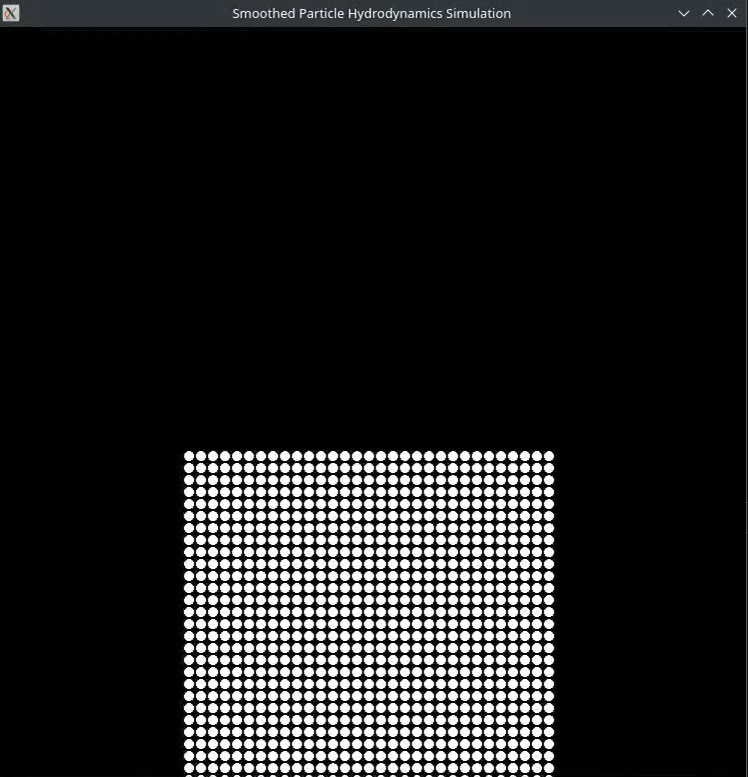
\includegraphics[width = 0.3\textwidth]{no_collision_f2.png}
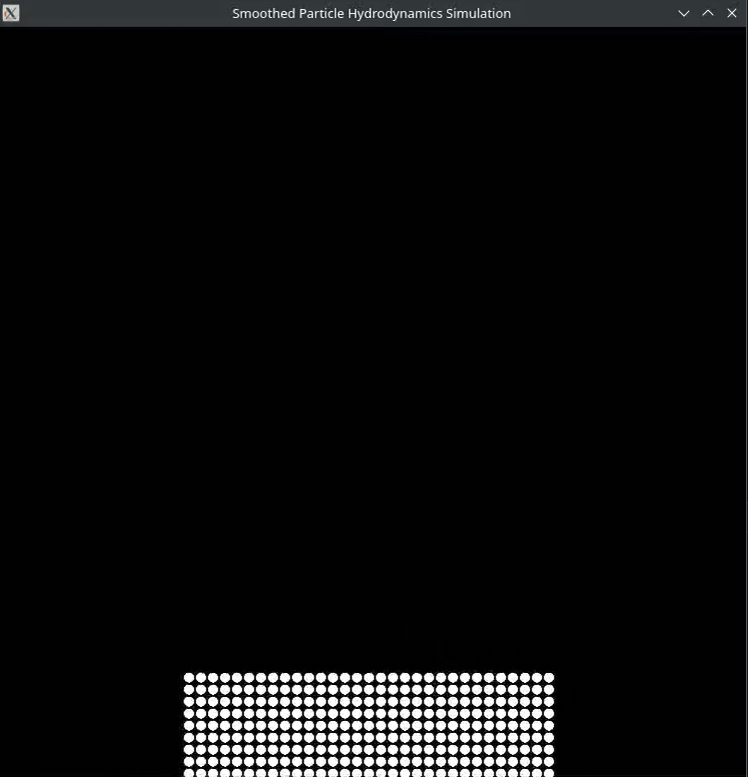
\includegraphics[width = 0.3\textwidth]{no_collision_f3.png}
\caption{Gravity with no collision with screen border.}
\label{fig:nograv}
\end{figure}

\begin{figure}[h]
\centering
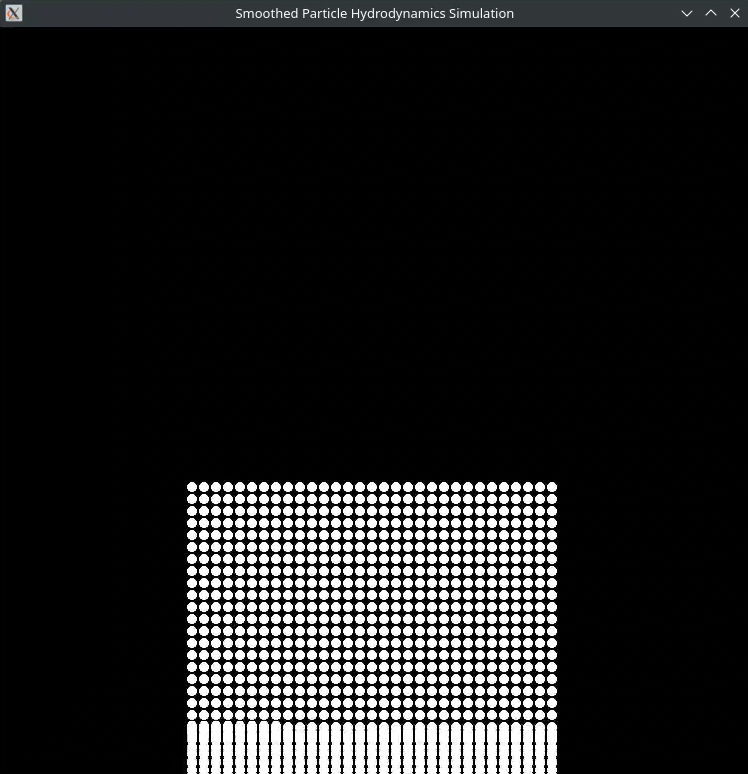
\includegraphics[width = 0.45\textwidth]{collision_f1.png}
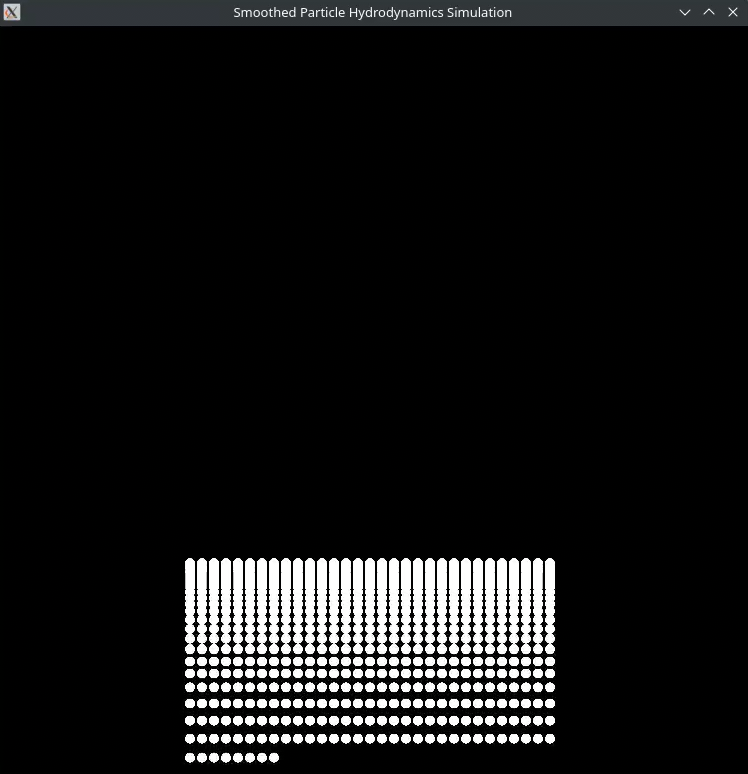
\includegraphics[width = 0.45\textwidth]{collision_f2.png}
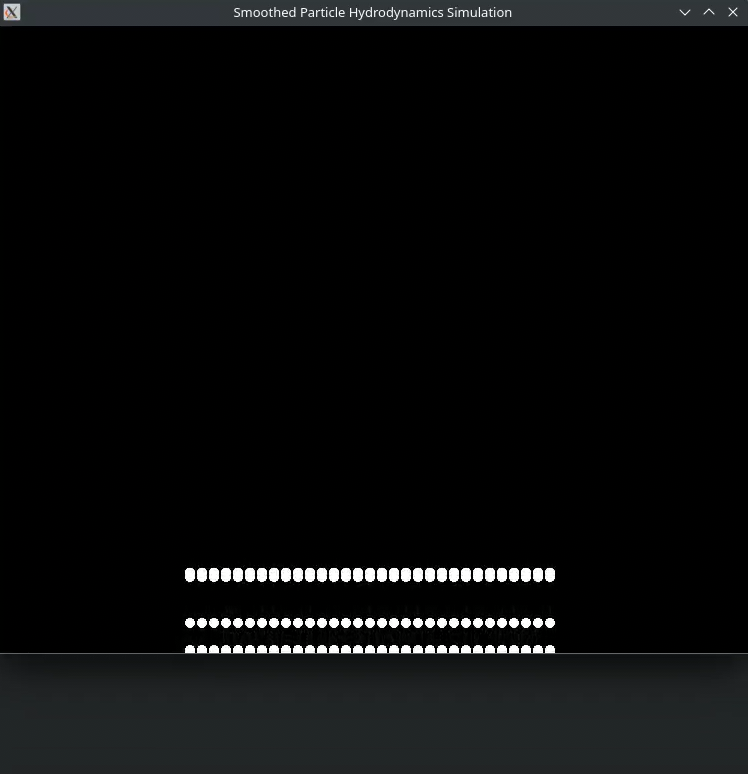
\includegraphics[width = 0.45\textwidth]{collision_f3.png}
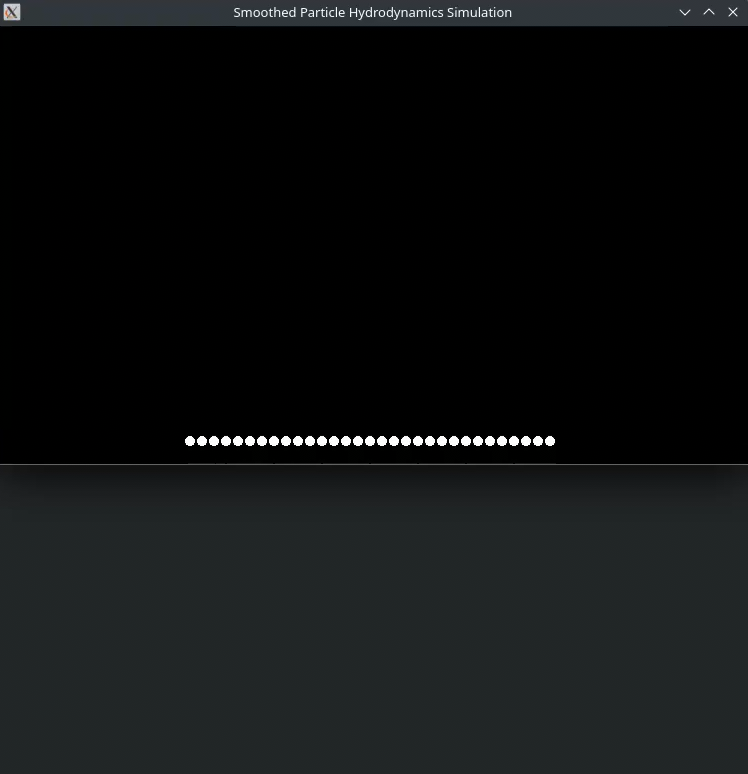
\includegraphics[width = 0.45\textwidth]{collision_f4.png}
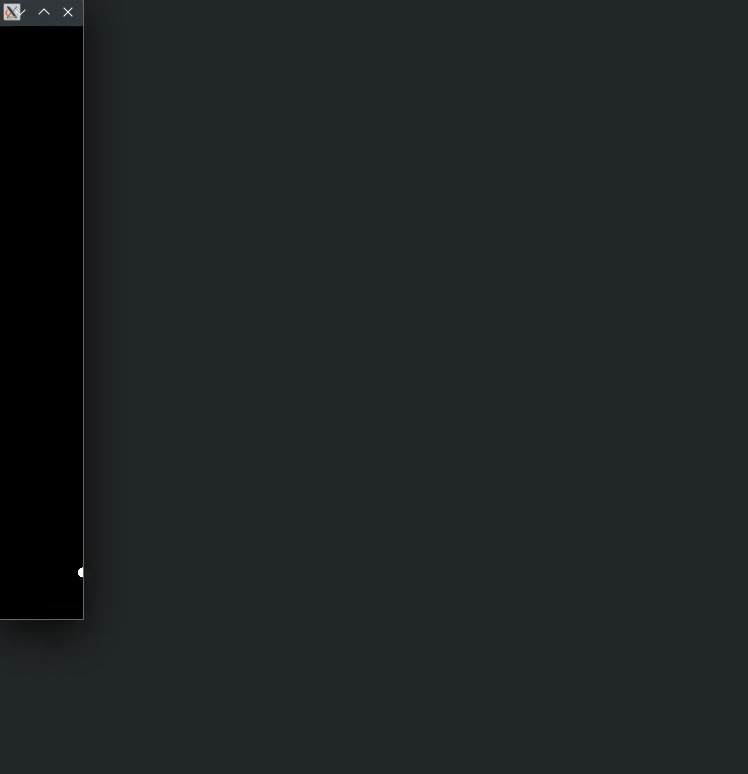
\includegraphics[width = 0.45\textwidth]{collision_f5.png}
\caption{Gravity with collision and window resizing.}
\label{fig:grav}
\end{figure}

\begin{figure}[h]
\centering
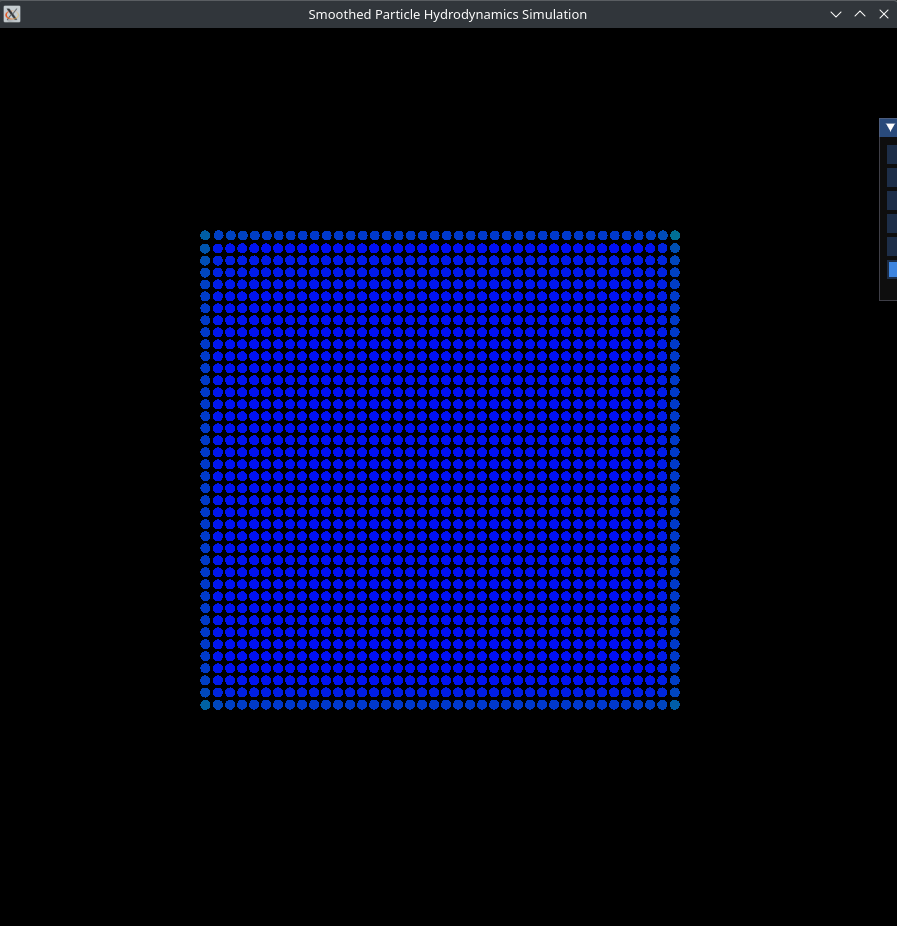
\includegraphics[width = 0.4\textwidth]{high_pressure.png}
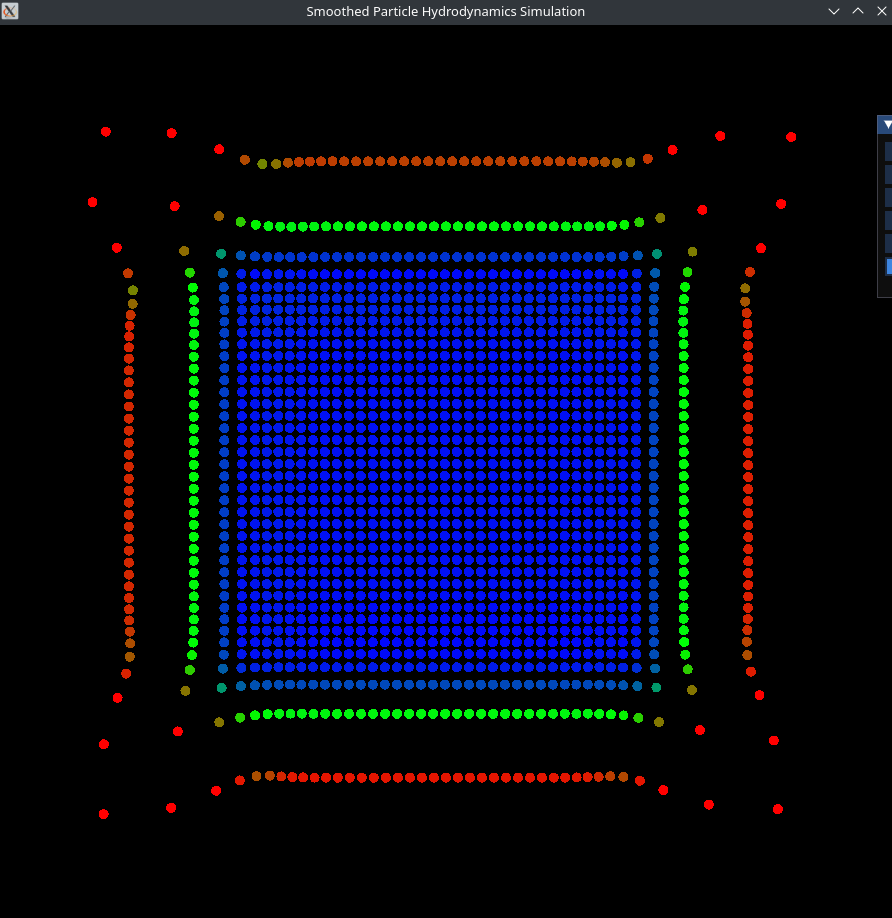
\includegraphics[width = 0.4\textwidth]{mid_pressure.png}
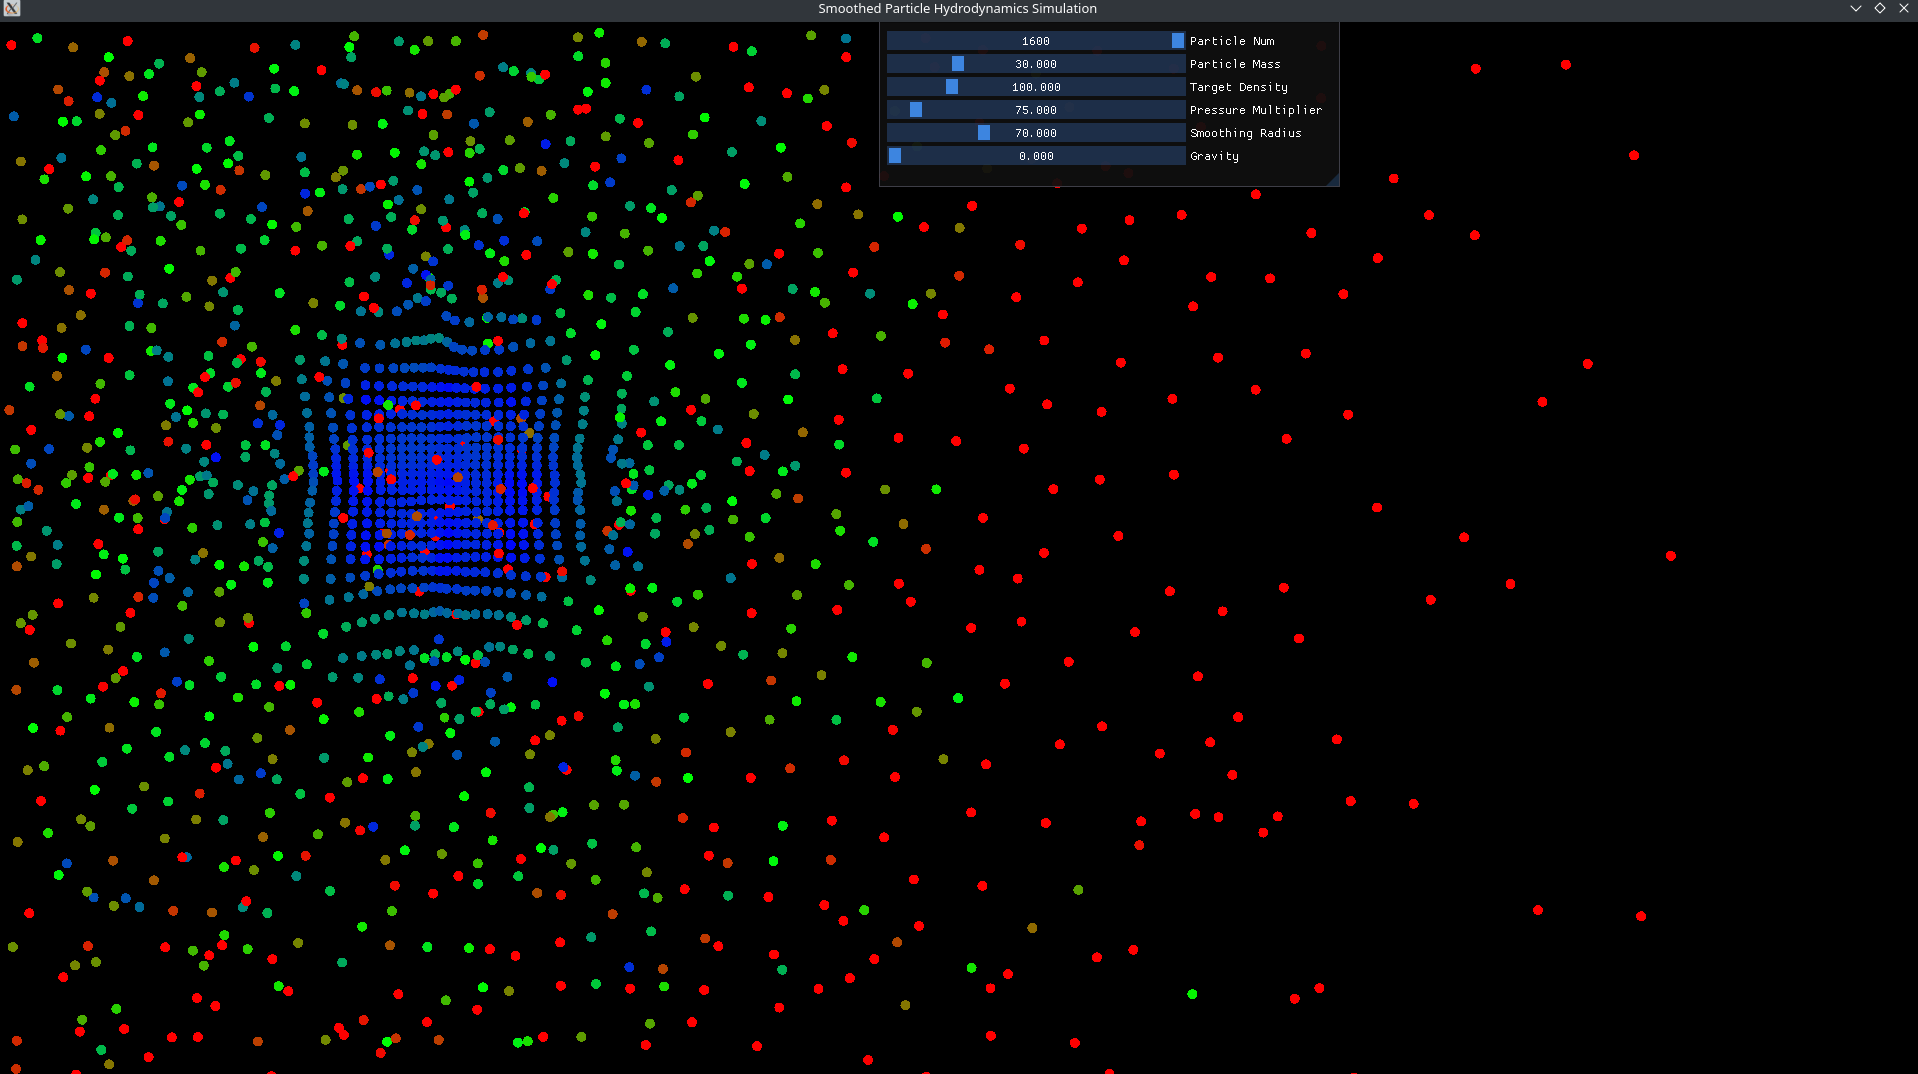
\includegraphics[width = 0.75\textwidth]{low_pressure.png}
\caption{Fluid particles moving down the pressure gradient.}
\label{fig:pressure_grad}
\end{figure}

\begin{figure}[h]
\centering
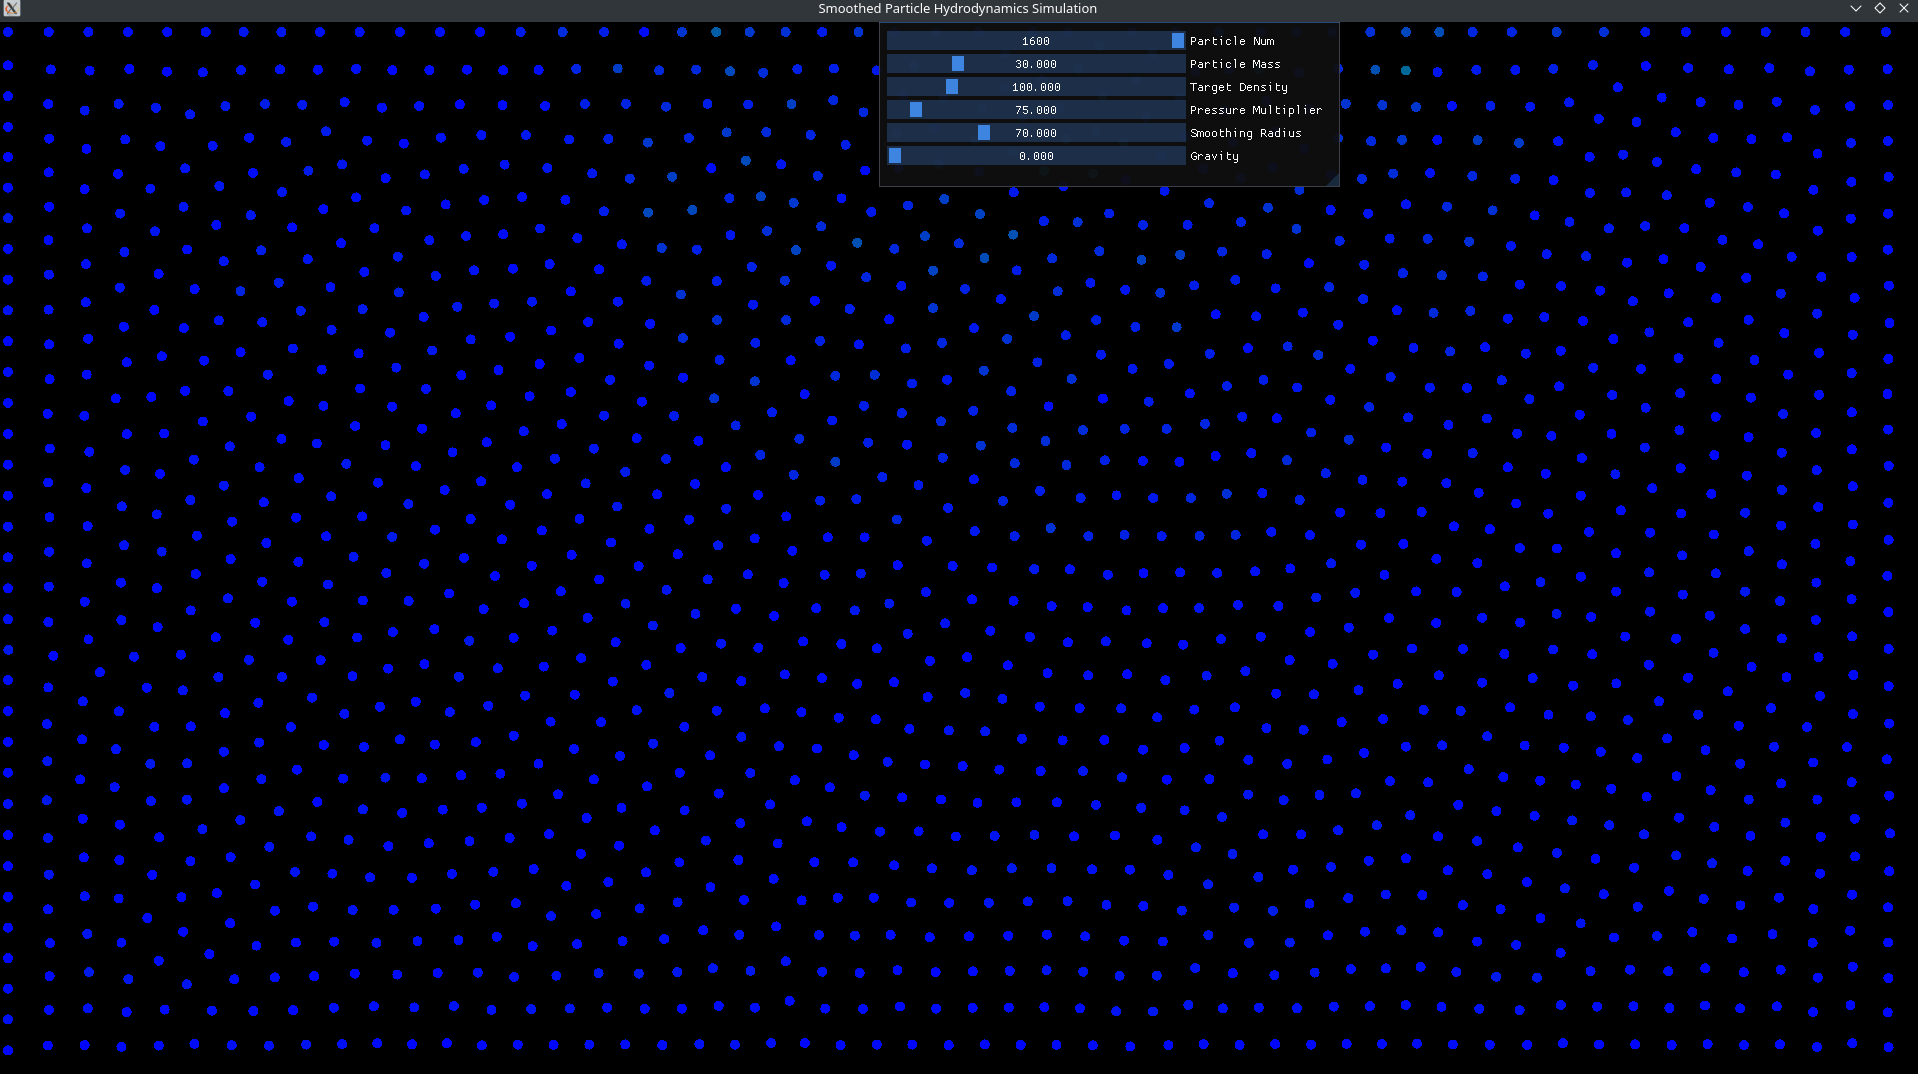
\includegraphics[width = 0.75\textwidth]{even_lower_pressure.png}
\caption{Fluid particles reaching a constant density in a stable state.}
\label{fig:constant_density}
\end{figure}

\begin{figure}[h]
\centering
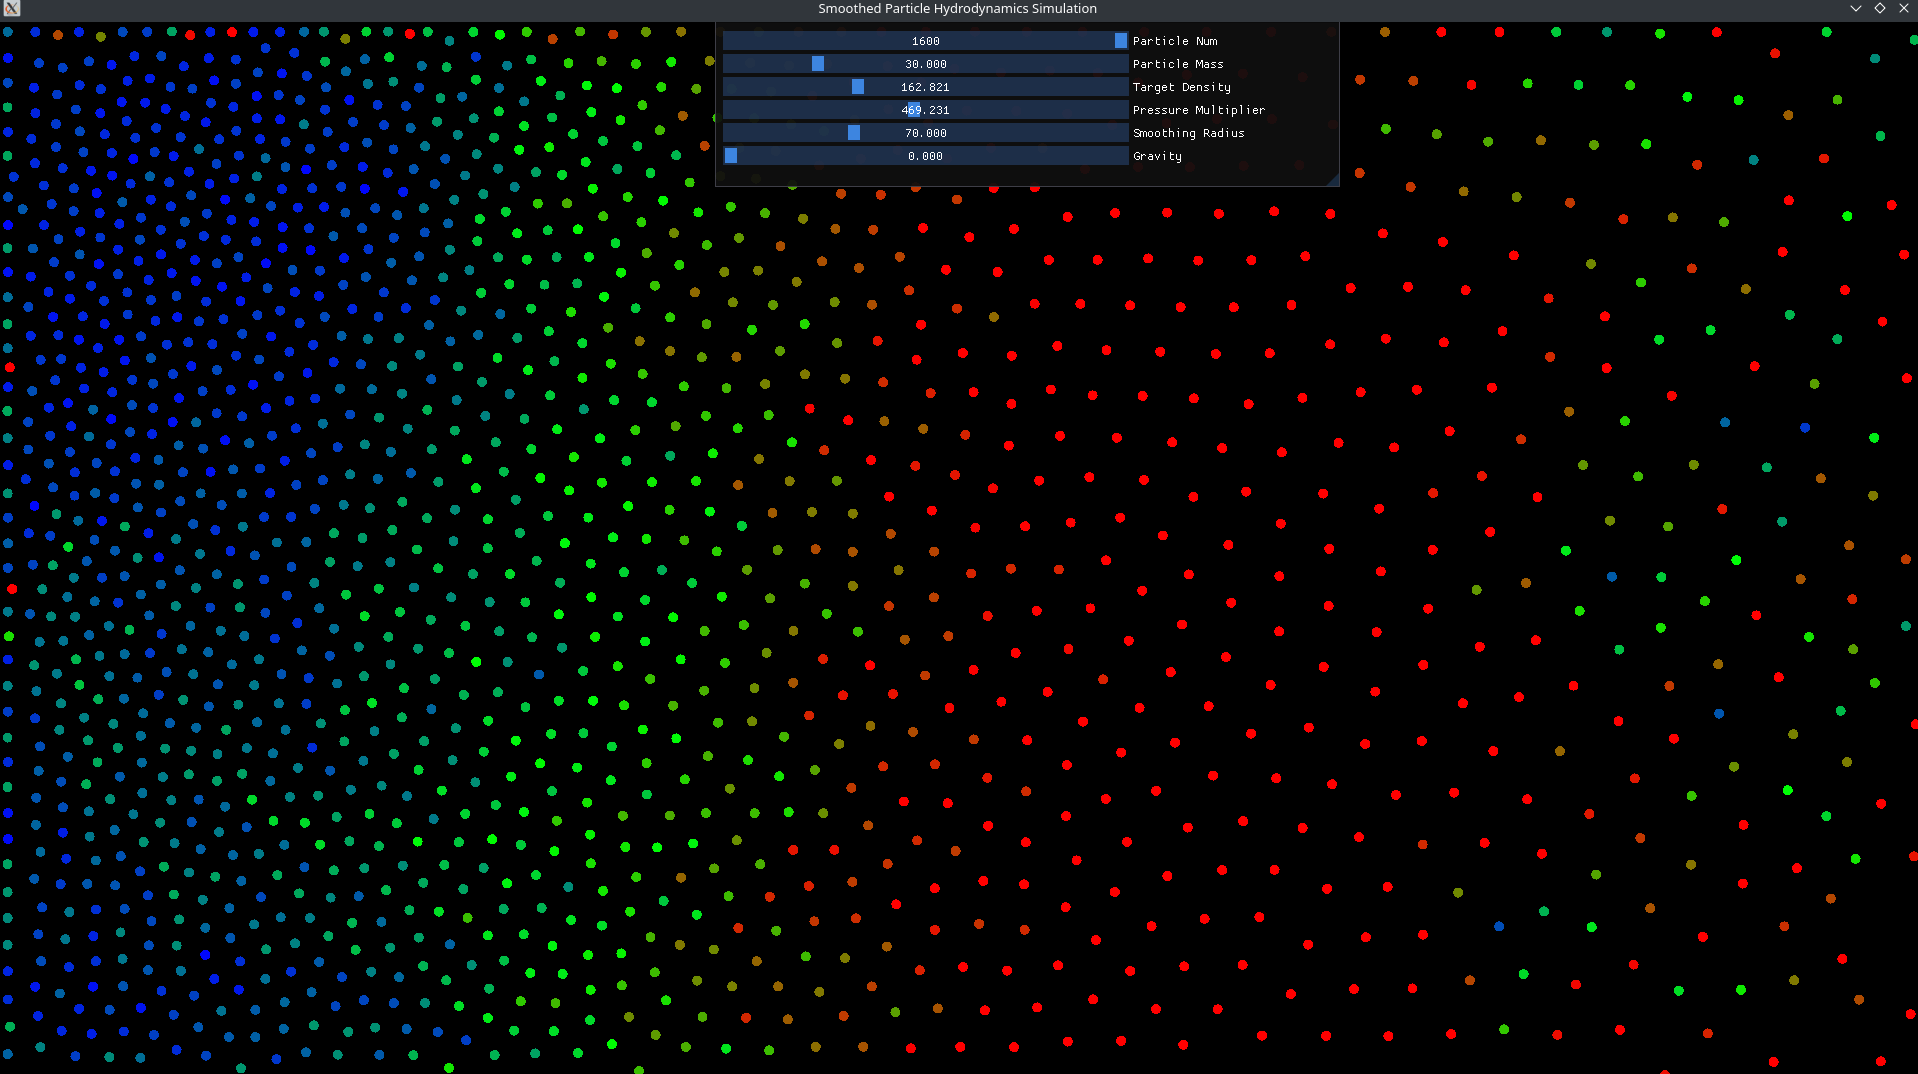
\includegraphics[width = 0.9\textwidth]{greenish_visco.png}
\caption{Red particles with high velocities becoming green at the edge, displaying viscosity}
\label{fig:viscosity}
\end{figure}

\begin{figure}[h]
\centering
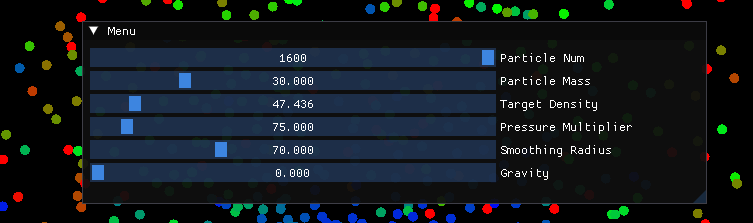
\includegraphics[width=1\textwidth]{sliders.png}
\caption{ImGui sliders on screen.}
\label{fig:sliders}
\end{figure}

\begin{figure}[h]
\centering
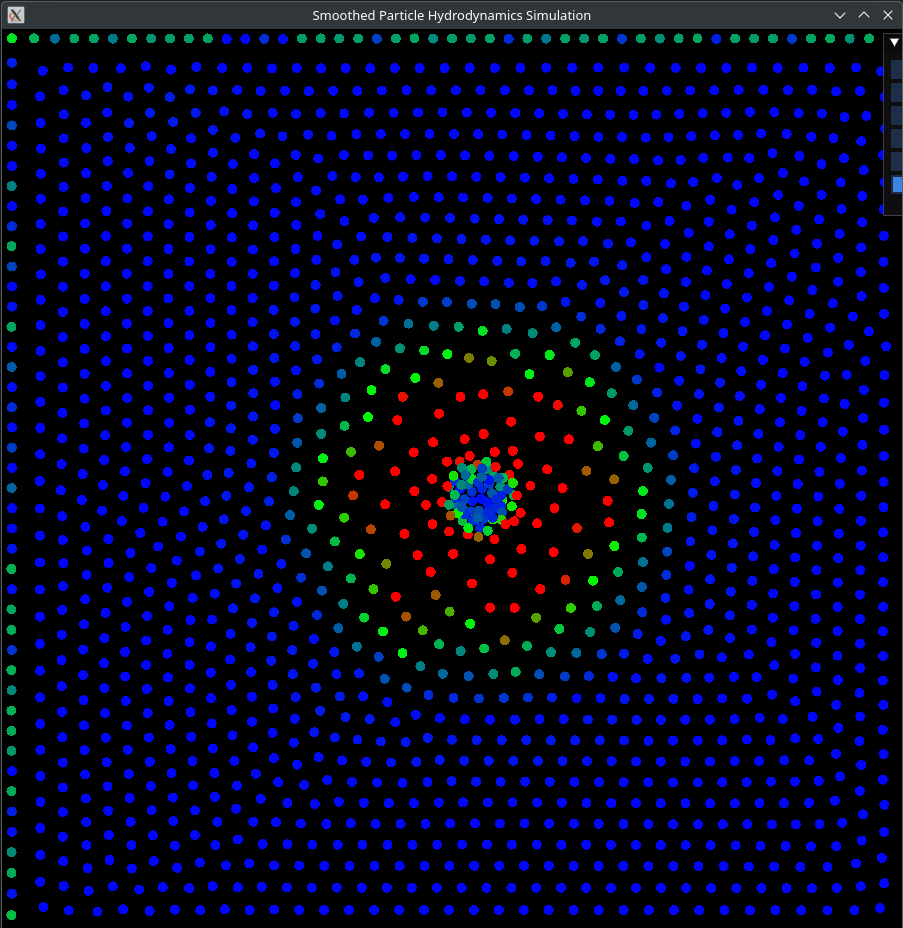
\includegraphics[width=0.4\textwidth]{attractive.png}
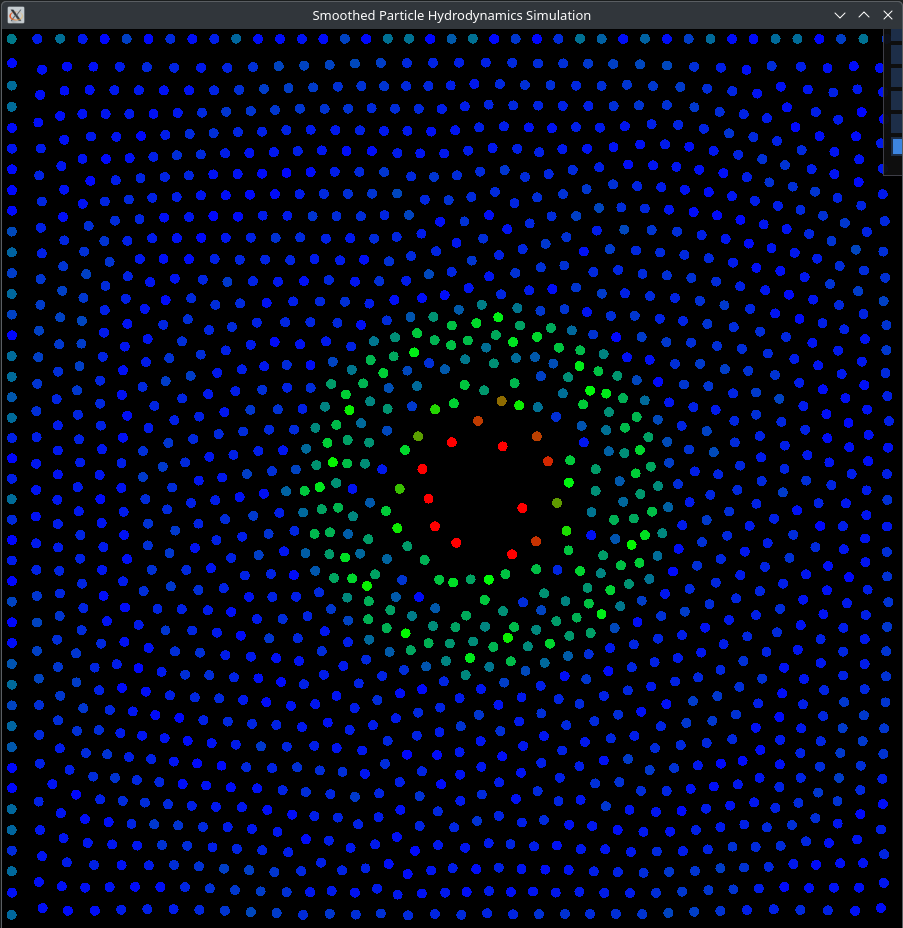
\includegraphics[width=0.4\textwidth]{repulsive.png}
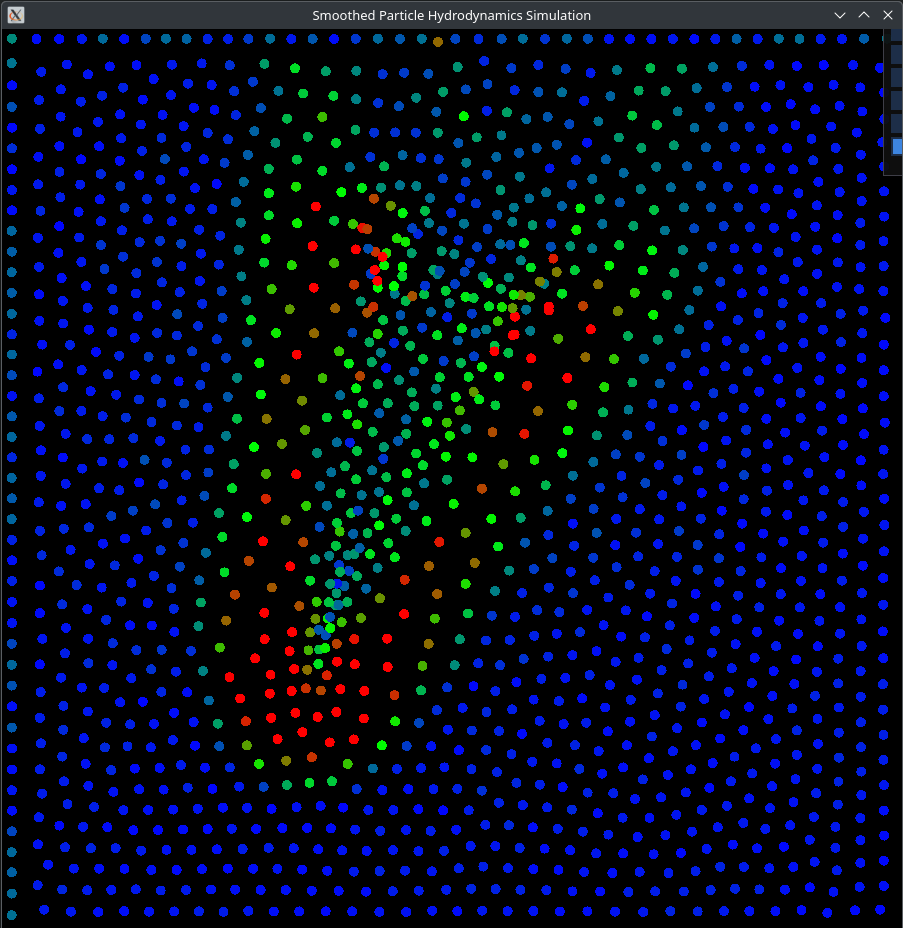
\includegraphics[width=0.75\textwidth]{mouse_drag.png}
\caption{Attractive and repulsive mouse forces with mouse drag effect.}
\label{fig:mouse_forces}
\end{figure}

\begin{figure}[h]
\centering
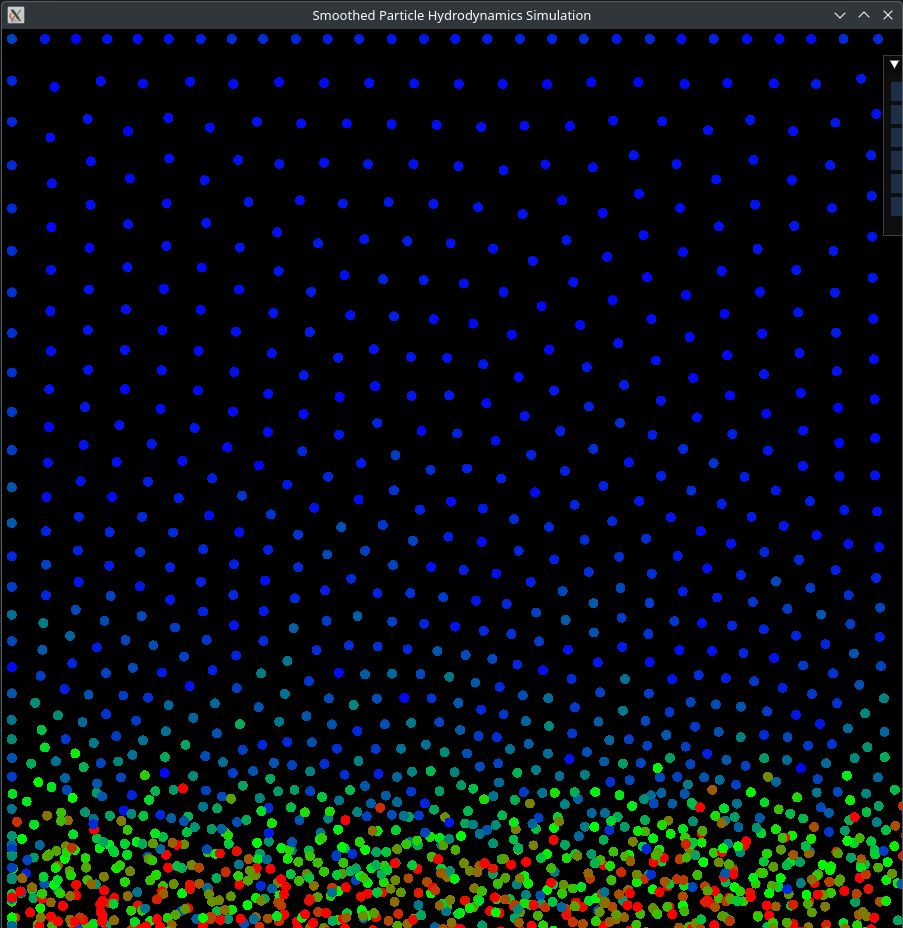
\includegraphics[width=1\textwidth]{heavy_gas.png}
\caption{Fluid with gravity behaving like a boiling liquid or heavy gas.}
\label{fig:heavy_gas}
\end{figure}

\begin{figure}[h]
\centering
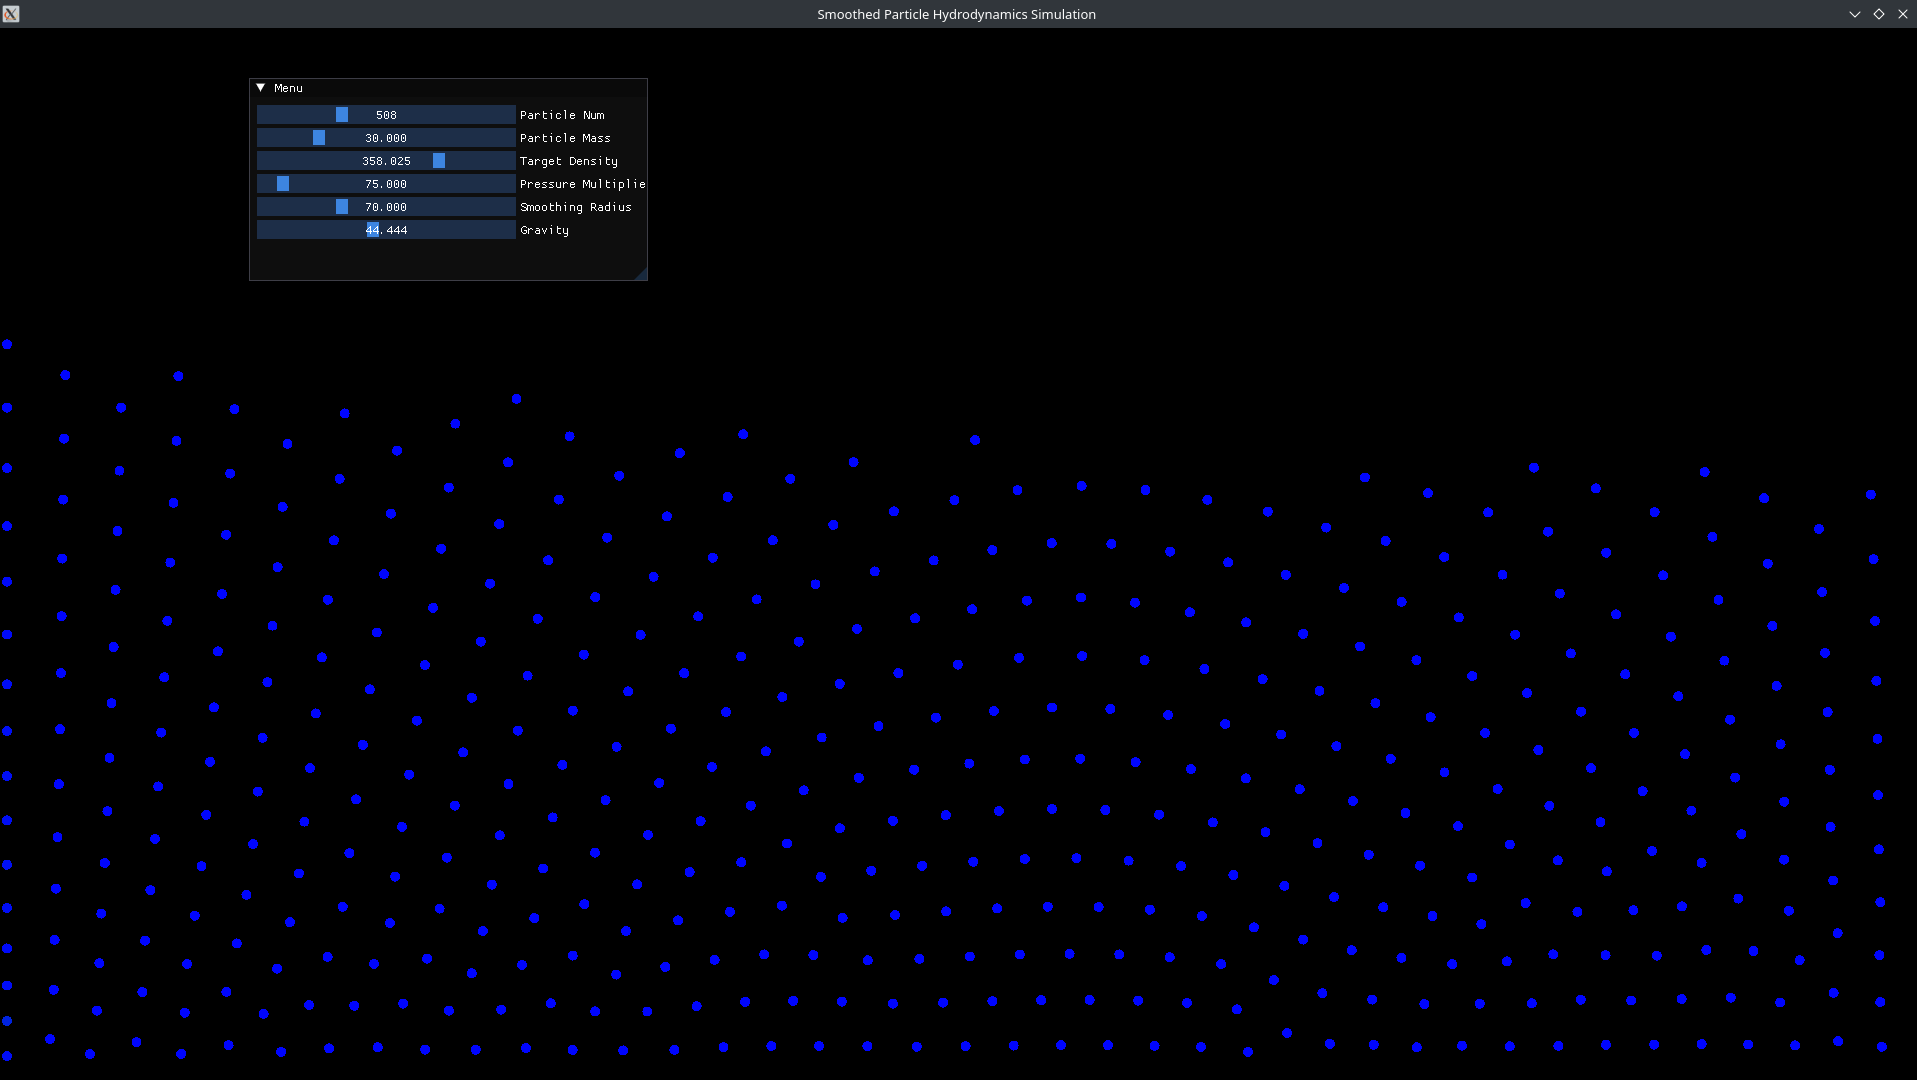
\includegraphics[width=1\textwidth]{jagged.png}
\caption{Fluid with gravity giving an unsmooth surface.}
\label{fig:jagged}
\end{figure}

\end{appendices}
\end{document}
